\documentclass[a4paper]{article}

\newif\ifdraft\drafttrue
\newif\ifinlineref\inlinereffalse
\newif\iffinal\finalfalse
\newif\ifextended\extendedfalse
\newif\ifdotikz\dotikzfalse
\newif\ifmakeallproofsinline\makeallproofsinlinefalse

% remove for inline references
%\inlinereftrue
% remove for submission and final version
\draftfalse
% remove for final version
\finaltrue
% remove for extended version
%\extendedtrue
% activate to show all proofs inline
% deactivate to show proofs where they are "located" (see macros below)
%\makeallproofsinlinetrue

% deactivate this to not compute in-line graphics
\dotikztrue
%
% activate above line and use the following to recompute in-line graphics
%   for j in $(egrep 'beginpgfgraphicnamed\{[^\{\}]*\}' abcmanual.tex | tr \{\} ' ' | awk '{print $2;}'); do pdflatex --jobname=$j abcmanual.tex ; mv $j.pdf figures/ ; done
%

\usepackage{color}
\usepackage{url}
\usepackage{geometry}
\usepackage[normalem]{ulem}

\usepackage{graphicx}
\graphicspath{{figures/}}

\ifdotikz
\usepackage{tikz}
\pgfrealjobname{abcmanual}
\usetikzlibrary{shapes,arrows,backgrounds,chains,%
matrix,patterns,arrows,decorations.pathmorphing,decorations.pathreplacing,%
positioning,fit,calc,decorations.text,shadows%
}
\else
\long\def\beginpgfgraphicnamed#1#2\endpgfgraphicnamed{\includegraphics{#1}}
\fi

\makeatletter
\pgfdeclareshape{document}{
	\inheritsavedanchors[from=rectangle] % this is nearly a rectangle
	\inheritanchorborder[from=rectangle]
	\inheritanchor[from=rectangle]{center}
	\inheritanchor[from=rectangle]{north}
	\inheritanchor[from=rectangle]{south}
	\inheritanchor[from=rectangle]{west}
	\inheritanchor[from=rectangle]{east}
	% ... and possibly more
	\backgroundpath{% this is new
		% store lower right in xa/ya and upper right in xb/yb
		\southwest \pgf@xa=\pgf@x \pgf@ya=\pgf@y
		\northeast \pgf@xb=\pgf@x \pgf@yb=\pgf@y
		\pgf@xc=\pgf@xb \advance\pgf@xc by-10pt % this should be a parameter
		\pgf@yc=\pgf@yb \advance\pgf@yc by-10pt
		% construct main path
		\pgfpathmoveto{\pgfpoint{\pgf@xa}{\pgf@ya}}
		\pgfpathlineto{\pgfpoint{\pgf@xa}{\pgf@yb}}
		\pgfpathlineto{\pgfpoint{\pgf@xc}{\pgf@yb}}
		\pgfpathlineto{\pgfpoint{\pgf@xb}{\pgf@yc}}
		\pgfpathlineto{\pgfpoint{\pgf@xb}{\pgf@ya}}
		\pgfpathclose
		% add little corner
		\pgfpathmoveto{\pgfpoint{\pgf@xc}{\pgf@yb}}
		\pgfpathlineto{\pgfpoint{\pgf@xc}{\pgf@yc}}
		\pgfpathlineto{\pgfpoint{\pgf@xb}{\pgf@yc}}
		\pgfpathlineto{\pgfpoint{\pgf@xc}{\pgf@yc}}
	}
}
\makeatother

\newcommand{\dlvhex}{{\sc dlvhex}}
\newcommand{\hex}{{\sc hex}}
\newcommand{\abcs}{{ABC}}

\begin{document}
	
	\title{The \abcs{} Benchmarking System}
	\author{Christoph Redl}

%	\maketitle

\begin{titlepage}
    \centering
    \vfill
	\newgeometry{margin=1in}
    \vskip2cm
        {\bfseries\Huge The \abcs{} Benchmarking System} \\[1em]
        {\bfseries\Huge User Manual} \\
        \vskip3.0cm
%        {\sc\Large INFSYS Research Report 1843-15-07} \\
        \medskip
        {\Large \today}        
        \vskip2cm
        {\bfseries\Large
        Christoph Redl \\
        }    
        \vspace{1cm}
        \begin{tabular}{c}
        {\Large}
          Institut f\"ur Informationssysteme,\\
          Abteilung Wissensbasierte Systems,\\
          Technische Universit\"at Wien, Austria \\
          {redl@kr.tuwien.ac.at} \\[1ex]
        \end{tabular}
        \vspace{4cm}
	\restoregeometry
\end{titlepage}
	
	\section{Introduction}
	\label{sec:introduction}

		This paper describes the \abcs{} benchmarking system
		for \uline{a}utomated \uline{b}enchmark runs on top of HT\uline{C}ondor, i.e.,
		comparing systems or system configurations to each other.
		The system is intended to be easy to use yet customizable to a large variety of
		benchmark problems.
		Although the system has originally been developed for the \hex-program reasoner \dlvhex{}\footnote{\url{http://www.kr.tuwien.ac.at/research/systems/dlvhex}},
		it was kept generic such that it can be used for experiments with other systems as well.
		The user is required to provide no more than one script for each benchmark problem,
		which essentially specifies problem-specific parameters and then delegates the call
		to generic scripts provided by this system.
		
		The \abcs-system
		is intended to run benchmark instances with multiple system configurations
		and extract benchmark parameters (such as grounding and solving time, number of answer sets) for each.
		It supports automated scheduling of instances, parameter extraction,
		aggregating the parameters,
		generating a table in text or \LaTeX{} format,
		and comparison of the results with previous runs.
		For scheduling benchmark instances, the system supports sequential runs using shell scripts only,
		or the HTCondor system\footnote{\url{http://research.cs.wisc.edu/htcondor}}.

	\section{Basic Usage of the System}
	\label{sec:usage}

		The system is implemented as a set of shell scripts which should work on most Linux shells; at least the \emph{bash} shell.
		The basic functions of the system do not have any further requirements, only features such as scheduling on top of HTCondor
		or aggregation of the results (see below) depend on third-party software.
		All scripts of the \abcs-system are collected in the directory {\tt scripts},
		to which we refer in the following whenever we discuss shell scripts.
		It is suggested to add the {\tt scripts} directory to the search path for executables.
		\footnote{While the \abcs{} system is generic and most scripts are useful for benchmarks with any software system,
		few are specific for the \dlvhex{} reasoner, which are easily recognizable by the prefix {\tt dlvhex\_} in their filenames.}

		In order to use the system for a concrete benchmark problem,
		the file {\tt run\_template.sh}
		has to be copied to {\tt run.sh} within the benchmark problem's directory.
		The file needs then to be adopted to the problem by modifying the lines
		marked with (1), (2) and (3) as follows.
		\begin{enumerate}
		\item[(1)] The loop condition which iterates over the instances of the benchmark needs to be configured.
			Usually this condition will iterate over files, but sometimes also an iteration in a certain range can be useful.

			\begin{tabbing}
				\textbf{Example: } \= {\tt "instances/*.hex"} \\
				\> iterates over all {\tt .hex} files in directory {\tt instances}.
			\end{tabbing}

			\begin{tabbing}
				\textbf{Example: } \= {\tt "\{1..20\}"} \\
				\> iterates over the integers from $1$ to $20$.
			\end{tabbing}
		\item[(2)] Here, the commands (e.g.~calls of a reasoner or another software systems) to be compared should be entered in a semicolon-separated list.

			When comparing entirely different systems,
			the configurations specified at (2) should contain the command strings \emph{including} the executable name and all options.

			\begin{tabbing}
				\textbf{Example: } \= {\tt "dlv;clasp;dlv -n=1;clasp -n=1"} \\
				\> compares {\sc DLV} and {\sc clasp} runs for computing \\
				\> all and the first ({\tt -n=1}) answer set, respectively.
			\end{tabbing}

			If all configurations compare the same system (e.g.~\dlvhex{}) but with different options,
			then as a shortcut the static part can (but does not need to) be part of the string at
			(3) (see below), while (2) may contain only the changing parts of the command.

			\begin{tabbing}
				\textbf{Example: } \= {\tt "flpcheck=explicit;--flpcheck=ufs"} \\
				\> compares two \dlvhex{} configurations, where the actual \\
				\> reasoner call is specified at (3) (see below).
			\end{tabbing}

		\item[(3)] Here, the static part of the actual shell command for a reasoner call needs to be inserted (i.e.,~without configuration-specific options).

			The tokens {\tt INST} and {\tt CONF}\footnote{
			Alternatively to {\tt INST} and {\tt CONF}, the meta-variables {\tt \textbackslash\$instance} and {\tt \textbackslash\$config}
			within the command string can be used (e.g.~{\tt dlvhex2 -n=1 \textbackslash\$config \textbackslash\$instance});
			note the backslash in front of the {\$} characters which makes sure that the variables are not immediately resolved but
			are part of the string and are to be resolved later when an individual instance and configuration is to be inserted.}
			will be substituted by the instance name and the current configuration, respectively.

			If the string at (2) contains full commands, then
			the string at (3) should be {\tt "CONF INST"}. Since {\tt CONF} in (3)
			will be substituted by the elements from the configuration string before executing the command, this will
			produce complete reasoner calls.

			\begin{tabbing}
				\textbf{Example: } \= Let {\tt "dlv;clasp;dlv -n=1;clasp -n=1"} be the \\
				\> configuration string at (2). \\
				\> Then the string {\tt "CONF INST"} at (3) will evaluate: \\
				\> \ \ \ {\tt dlv INST} \\
				\> \ \ \ {\tt clasp INST} \\
				\> \ \ \ {\tt dlv -n=1 INST} \\
				\> \ \ \ {\tt clasp -n=1 INST} \\
				\> for all instances {\tt INST}.
			\end{tabbing}

			If the string at (2) contains only the changing part of the command,
			then the static part must contained in the string at (3).

			\begin{tabbing}
				\textbf{Example: } \= Let {\tt "flpcheck=explicit;--flpcheck=ufs"} be the \\
				\> configuration string at (2). \\
				\> Then the string {\tt "dlvhex2 -n=1 CONF INST"} at (3) will evaluate: \\
				\> \ \ \ {\tt dlvhex2 -n=1 --flpcheck=explitit INST} \\
				\> \ \ \ {\tt dlvhex2 -n=1 --flpcheck=ufs INST} \\
				\> for all instances {\tt INST}.
			\end{tabbing}
		\end{enumerate}
		
		Note that the scripts {\tt runinsts.sh} and {\tt runconfigs.sh} support more
		parameters than shown in {\tt run\_template.sh}.
		However, the default values are good for most benchmarks.
		If the aggregation of the results or
		the extraction of benchmark parameters from the runs needs to be customized,
		then Section~\ref{sec:architecture} is a good starting point to learn about the parameters.
		
		As stated above, it is convenient to add the path to the {\tt scripts} directory to the {\tt PATH} variable.
		In this case, scheduling the benchmark instances is possible by simply calling {\tt ./run.sh},
		otherwise the path to this directory needs to be passed as parameter to {\tt run.sh}
		(cf.~Section~\ref{sec:architecture:run}).

		Moreover, the beginnings of {\tt run.sh} scripts are in many cases exactly
		like in {\tt run\_template.sh}. Thus this part can be directly imported by
		\begin{center}
			{\tt source run\_header.sh}
		\end{center}
		provided that the benchmark script directory is the {\tt PATH} variable.
		This also defines the aliases
		{\tt all=$0$}, {\tt instance=\$2}, {\tt to=\$3}, {\tt bmscripts=\$4}
		if {\tt \$1} is {\tt single}, and
		{\tt all=1}, {\tt to=\$2}, {\tt bmscripts=\$3} otherwise (cf.~Section~\ref{sec:architecture:run}).
		Moreover, {\tt mydir} will be set to the absolute path of the directory where
		the current {\tt run.sh} script is located and {\tt req} to the requirements file to be used.
			
	\section{System Architecture and Customization}
	\label{sec:architecture}

		The basic system architecture is visualized in Figure~\ref{fig:architecture}.
		There is a single benchmark-specific file {\tt run.sh}, which is usually stored
		in the benchmark's directory (different from the {\tt scripts} directory of the \abcs-system).
		This file can be used for scheduling all instances and for evaluating a single instance
		(controlled by parameters). Normally, the user calls this file without any parameters,
		which schedules all instances (due to the default values for the parameters).
		Internally, {\tt run.sh} uses scripts from the benchmark scripts directory
		({\tt runinsts.sh} and {\tt runconfigs.sh}; those are not benchmark-specific) to schedule all instances for all configurations
		which are to be compared. Those scripts will make callbacks to {\tt run.sh} for evaluating single instances
		(appropriate parameters make this script run a single instance rather than all instances in the initial call).
		Note that the two {\tt run.sh} occurrences in Figure~\ref{fig:architecture} refer
		to a single physical file (symbolized by their connection).
		
		For each finished instance, the script system will call an \emph{output builder}
		which extracts the actual benchmark parameters the user is interested in,
		e.g.~time information and number of answer sets,
		from the reasoner output (standard output and standard error).
		The result is stored in a separate result file for each instance.
		When all instances have finished, the script system further calls an \emph{aggregation script},
		which generates the final benchmark table from the results of individual instances.
		The script system provides a standard output builder {\tt outputbuilder.sh} and a standard aggregation script {\tt aggregateresults.sh},
		which are good for many benchmark problems, but customization is possible by providing alternative scripts
		(which need to be specified within {\tt run.sh} as described in Sections~\ref{sec:architecture:runinsts} and~\ref{sec:architecture:runconfigs}).

		\begin{figure}
			\centering
			\beginpgfgraphicnamed{architecture}
			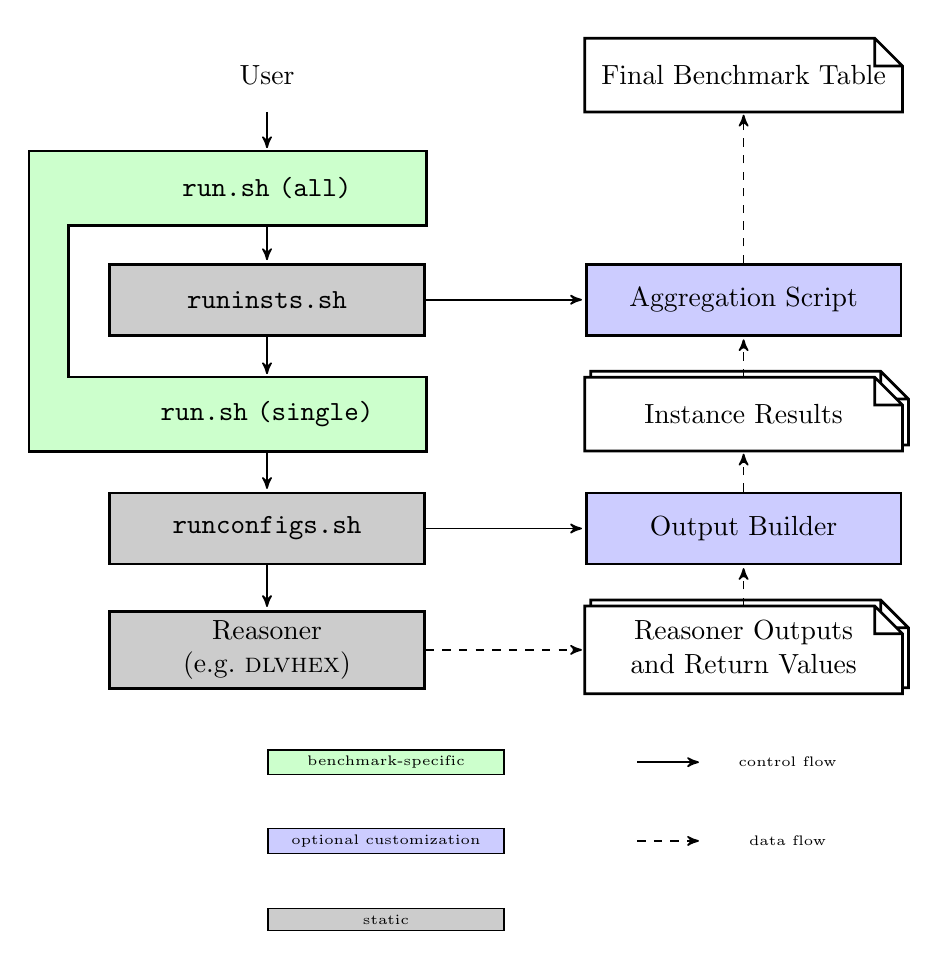
\begin{tikzpicture}[->,>=stealth',shorten >=1pt,auto,node distance=1.0cm,semithick]
				\matrix(m)[matrix of nodes,row sep=0.5cm,column sep=2cm,
					nodes={draw, % General options for all nodes
					  line width=1.0pt,
					  anchor=center, 
					  text centered,
					  minimum width=4.0cm,
					  minimum height=9mm
					},
					empty/.style={
						line width=1.25pt,
						text width=3.5cm, 
						minimum height=9mm,
						draw=none
					},
					bmspecificscript/.style={
						line width=1.25pt,
						text width=3.5cm, 
						minimum height=9mm,
						fill=green!20
					},
					staticscript/.style={
						line width=1.0pt,
						text width=3.5cm, 
						minimum height=9mm,
						fill=black!20
					},
					customizeablescript/.style={
						line width=1.0pt,
						text width=3.5cm, 
						minimum height=9mm,
						fill=blue!20
					},
					user/.style={
						draw=none
					}
				]{
					|[user]| User & |[document]| Final Benchmark Table \\
					|[empty]| \tt run.sh (all) & \\
					|[staticscript]| \tt runinsts.sh & |[customizeablescript]| Aggregation Script \\
					|[empty]| \tt run.sh (single) & |[document,copy shadow,fill=white]| Instance Results \\
					|[staticscript]| \tt runconfigs.sh & |[customizeablescript]| Output Builder \\
					|[staticscript]| Reasoner (e.g.~{\sc dlvhex}) & |[document,copy shadow,fill=white]| \begin{tabular}{c}Reasoner Outputs \\ and Return Values\end{tabular} \\
				};

				{
					\tiny
	        		\node[draw,fill=green!20,below=2.5cm of m-5-1,minimum width=3.0cm,anchor=west] (lbsc) {benchmark-specific};
	        		\node[draw,fill=blue!20,below of=lbsc,minimum width=3.0cm] (lcs) {optional customization};
	        		\node[draw,fill=black!20,below of=lcs,minimum width=3.0cm] (lss) {static};
	        		\node[right=1.5cm of lbsc] (ls1) {}; \node[right of=ls1] (ls2) {}; \node[right of=ls2] (ls3) {control flow};
	        		\path[draw,->] (ls1) -- node {} (ls2);
	        		\node[below of=ls1] (ld1) {}; \node[right of=ld1] (ld2) {}; \node[right of=ld2] (ld3) {data flow};
	        		\path[draw,->,dashed] (ld1) -- node {} (ld2);
				}

				\path[draw,->] (m-1-1) -- node {} (m-2-1);
				\path[draw,->] (m-2-1) -- node {} (m-3-1);
				\path[draw,->] (m-3-1) -- node {} (m-4-1);
				\path[draw,->] (m-4-1) -- node {} (m-5-1);
				\path[draw,->] (m-5-1) -- node {}  (m-5-2);
				\path[draw,->,dashed] (m-5-2) -- node {} (m-4-2);
				\path[draw,->,dashed] (m-4-2) -- node {} (m-3-2);
				\path[draw,->,dashed] (m-3-2) -- node {} (m-1-2);
				\path[draw,->] (m-3-1) -- node {} (m-3-2);
				\path[draw,->,dashed] (m-6-2) -- node {} (m-5-2);
				\path[draw,->] (m-5-1) -- node {} (m-6-1);
				\path[draw,->,dashed] (m-6-1) -- node {} (m-6-2);

				\begin{pgfonlayer}{background}
					\path[draw,fill=green!20,-,line width=1.0pt] (m-2-1.south east) -- (m-2-1.north east) -- ($(m-2-1.north west) - (1cm,0)$) -- ($(m-4-1.south west) - (1cm,0)$) -- (m-4-1.south east) -- (m-4-1.north east) -- ($(m-4-1.north west) - (0.5cm,0)$) -- ($(m-2-1.south west) - (0.5cm,0)$) -- (m-2-1.south east) -- (m-2-1.north east);
				\end{pgfonlayer}
			\end{tikzpicture}
		\endpgfgraphicnamed
			
		\caption{\abcs{} Benchmarking System Architecture}
		\label{fig:architecture}
		\end{figure}

		The following subsections describe the scripts of the benchmark system
		in more detail.
		Note that except for {\tt run\_template.sh}, which serves as an example
		for writing a benchmark-specific file {\tt run.sh}, none of these files need
		to be modified by the user.

		\subsection{\tt run\_template.sh}
		\label{sec:architecture:run}
		
			This file is an example for an implementation of {\tt run.sh}.
		    It specifies how to execute a single instance under various configurations
		    and how to iterate over the instances of the benchmark.
		    
		    The parameters mainly specify whether to execute all instances
		    of the benchmark (using further scripts from the \abcs{} benchmark system)
		    or a single instance.
		    Note that this script is (indirectly) recursively called:
		    usually, the first call is to evaluate all instances, which internally
		    calls {\tt runinsts.sh}, which in turn makes another (recursive) call of {\tt run.sh}
		    for evaluating every single instance.
		    A single instance is then usually evaluated under a number of configurations,
		    for which the script {\tt runconfigs.sh} is available.

		    However, this recursion is managed by the benchmark system.
		    The user only needs to adopt {\tt run.sh} as described in Section~\ref{sec:usage}.
		
		    \medskip\noindent{\bf Parameters:}
		    \begin{itemize}
				\item[{\tt \$1}:] (optional) {\tt all}, {\tt allseq} or {\tt single}, default is {\tt all}.
					\begin {itemize}
						\item If {\tt \$1} is {\tt all} then the instances are evaluated in parallel using HTCondor (which, obviously, needs to be installed in this case). There are no further mandatory parameters.
							\begin{itemize}
								\item[{\tt \$2}:] (optional) Timeout in seconds, default is $300$.
								\item[{\tt \$3}:] (optional) Directory with the benchmark scripts.
							\end{itemize}
						\item If {\tt \$1} is {\tt allseq} then the instances are evaluated sequentially. There are no further mandatory parameters.
							\begin{itemize}
								\item[{\tt \$2}:] (optional) Timeout in seconds, default is $300$.
								\item[{\tt \$3}:] (optional) Directory with the benchmark scripts.
							\end{itemize}
						\item If {\tt \$1} is {\tt single} then a single instance is evaluated. There are three more parameters, one of which is optional:
							\begin{itemize}
								\item[{\tt \$2}:] Instance name.
								\item[{\tt \$3}:] Timeout in seconds.
								\item[{\tt \$4}:] (optional) Directory with the benchmark scripts.
							\end{itemize}
					\end{itemize}
		    \end{itemize}
				
		\subsection{\tt runinsts.sh}
		\label{sec:architecture:runinsts}
		
		    This script implements a loop over instances and schedules them for execution,
		    which is done either sequentially or in parallel using HTCondor.
		    It is usually called from {\tt run.sh} of a concrete benchmark problem.
		    
		    The parameters of the script control the loop condition
		    and the command used for executing a single instance.
		    This script will also call the aggregation script (cf.~Section~\ref{sec:architecture:aggregate})
		    after execution of all instance
		    to produce the final benchmark table.
				
		    \medskip\noindent{\bf Parameters:}
		    \begin{itemize}
				\item[{\tt \$1}:] (optional) Instance loop condition, default is {\tt *.hex}.
				\item[{\tt \$2}:] (optional) Single benchmark command, default is {\tt ./run.sh}.
				\item[{\tt \$3}:] (optional) Working directory, default is {\tt \$PWD}.
				\item[{\tt \$4}:] (optional) Timeout in seconds, default is {\tt $300$}.
				\item[{\tt \$5}:] (optional) Custom aggregation script, default is {\tt aggregateresults.sh}
					in the {\tt scripts} directory of the \abcs{} system.
					Custom aggregation scripts need to behave as described in Section~\ref{sec:architecture:aggregate}.
				\item[{\tt \$6}:] (optional) Name of the benchmark, default is the name of the working directory.
				\item[{\tt \$7}:] (optional) Requirements file (cf.~Section~\ref{sec:architecture:reqfile}).
		    \end{itemize}
		 
		 	When the script makes a call for executing a single benchmark instance
		 	as specified by {\tt \$2}, it will run
		 	\begin{center}
		 		{\tt \$2 single INST TO SCRIPTS},
		 	\end{center}
		 	where {\tt INST} is the current instance (an element of the loop specified in {\tt \$1}),
		 	{\tt TO} is the timeout specified in {\tt \$4}
		 	and {\tt SCRIPTS} is the path of the benchmark scripts directly.
				
		\subsection{\tt runconfigs.sh}
		\label{sec:architecture:runconfigs}
		
		    This script implements the evaluation of
		    a single instance under various configurations.
		    It is usually called from {\tt run.sh} of a concrete benchmark problem
		    that needs to evaluate a single instance.
		
		    The parameters control the configurations to be compared
		    and the name of an output builder.
		
		    \medskip\noindent{\bf Parameters:}
		    \begin{itemize}
				\item[{\tt \$1}:] Command for executing an instance, which may contain the constant {\tt CONF} as a placeholder
					for options to be inserted and {\tt INST} as a placeholder for the instance.
				\item[{\tt \$2}:] A semicolon-separated list of configuration strings to be substituted for {\tt CONF} in {\tt \$1}.
				\item[{\tt \$3}:] Instance to be inserted in the command string in {\tt \$1} for {\tt INST}.
				\item[{\tt \$4}:] Timeout in seconds.
				\item[{\tt \$5}:] (optional) Custom output builder name of a script to build the output of a run, which gets the parameters, default is {\tt timeoutputbuilder.sh}
					in the {\tt scripts} directory of the \abcs{} system. A custom output builder needs to behave as described in Section~\ref{sec:architecture:outputbuilder}.
		    \end{itemize}
	
		\subsection{Output Builders}
		\label{sec:architecture:outputbuilder}
				
			An output builder is a script which extracts the actual benchmark parameters
			from a run. This is the information the user is interest in. Usually it
			includes timing information (e.g.~grounding and solving time), the number of answer sets, etc.
			
			An output builder gets the following parameters:
			    \begin{itemize}
					\item[{\tt \$1}:] Return value of the reasoner call ($0$ if success, $124$ if timeout, any other value $\not= 0$ if failed).
					\item[{\tt \$2}:] File with the overall runtime of the reasoner call.
					\item[{\tt \$3}:] File with standard output of the reasoner call.
					\item[{\tt \$4}:] File with standard error of the reasoner call.
			    \end{itemize}
			
			The output builder needs to return $0$ if it succeeded (note that the output builder can succeed in extracting information even if the reasoner failed!)
			and $\not=0$ if the output builder itself failed.
			
			It further needs to write a space-separated list of the actual benchmark parameters to standard output.
			This is usually a list of numbers to represent timing information, timeouts, number of answer sets, etc. For time values,
			the special values {\tt ---} and {\tt ===} for representing timeouts and memory outs, respectively, are supported.
			If {\tt ---} or {\tt ===} is output for some columns, the output builder can still return $0$, i.e.,
			output building counts as succeeded.
			In contrast, if the output builder completely fails to extract some information, it should output {\tt FAIL} for the according column
			and return $\not=0$; detailed error descriptions are allowed on standard error.
			
			The benchmark script directory provides the following predefined output builders:
					
			\begin{itemize}
			    \item {\tt timeoutbuilder.sh} extracts the overall time (one time column and a column $0/1$ for tagging successful/timeout instances).
			    \item {\tt gstimeoutbuilder.sh} extracts the overall time, the grounding and the solving time (each accompanied by a column $0/1$ for tagging successful/timeout instances).
			    \item {\tt ansctimeoutputbuilder.sh} extracts the overall time (accompanied by a column $0/1$ for tagging successful/timeout instances) and the number of answer sets.
                            \item {\tt debugoutbuilder.sh} is the same as {\tt timeoutputbuilder.sh} but includes also stdout and stderr of the command in the stderr of the benchmark results.
			\end{itemize}
	
		\subsection{Aggregation Scripts}
		\label{sec:architecture:aggregate}

			An aggregation script
		    generates the final output of a benchmark as a table in text format,
		    given the results of individual instances.
			This step requires the \emph{statistics system R}\footnote{\url{https://www.r-project.org}} to be installed.
		    As standard input the file gets the concatenation of the results for all instances produced by the output builder (cf.~Section~\ref{sec:architecture:outputbuilder}).
	
			In the input, column 1 is interpreted as instance size. The script is expected to aggregate
			over all instances of the same size and to output a single row for each instances size.
	
			Note that a custom aggregation script only needs to read from standard input and write to standard output
			and is not expected to interpret any parameters.
			However,
			the default aggregation script {\tt aggregateresults.sh} in the {\tt scripts} directory of the \abcs{} system
			provies some optional parameters, which allow in many cases to write custom aggregation scripts
			that simply delegate the call to the default one with appropriate parameters.
	
		    \medskip\noindent{\bf Parameters:}
		    \begin{itemize}
				\item[{\tt \$1}:] (optional) Timeout value (in seconds) to be used for {\tt ---} and {\tt ===} instances.
				\item[{\tt \$2},{\tt \$3}:] (optional) Start position and length of instance size information in the instance filenames (index origin $0$),
					or $0$ and $0$ for auto-detection, default is auto-detection.
				\item[{\tt \$4}:] (optional) Comma-separated list of column indexes to compute means.
				\item[{\tt \$5}:] (optional) Comma-separated list of column indexes to compute maxima.
				\item[{\tt \$6}:] (optional) Comma-separated list of column indexes to minima.
				\item[{\tt \$7}:] (optional) Comma-separated list of column indexes to sums.
		    \end{itemize}
	
			The default for {\tt \$4-\$7}
			is to compute means of odd and sums of even columns (interpreted as times and timeouts, respectively).
	
			If a customized aggregation script is specified in the call of {\tt runinsts.sh} (cf.~Section~\ref{sec:architecture:runinsts}),
			then this script can delegate the call to the default script {\tt aggregateresults.sh} with appropriate parameters.
	
		\subsection{Requirements File}
		\label{sec:architecture:reqfile}
				
			The requirements file specifies the hardware resources to be allocated
			for the benchmark run.
			An example is available in {\tt req\_template}.
			
			The file is roughly a resource specification to be added to
			HTCondor job files\footnote{\url{http://research.cs.wisc.edu/htcondor/}}.
			In addition, the following specification may be part of a resource file:
			\begin{itemize}
				\item {\tt \# sequential} \\
					Evaluate all instances in sequence (not using HTCondor).
				\item {\tt \# ExtendedNotification = mail@address.com} \\
					 Send the benchmark results by e-mail. 
			\end{itemize}
			Remark: The leading {\#} is important to make sure that HTCondor ignores these lines
			as they are not valid HTCondor syntax. However, the script system will still interpret them.
	
			The script system will use as requirements file the first one of the following which exists:
			\begin{enumerate}
				\item The file passed as argument {\tt \$7} to {\tt runinsts.sh}.
				\item The file {\tt req} in the same directory as the {\tt run.sh} script.
				\item The file {\tt req} in the {\tt scripts} directory of the \abcs{} system.
			\end{enumerate}

	\section{Advanced Features}
	\label{sec:advanced}

		This section discusses the advanced features of the benchmark system,
		which are needed for table formatting and comparison of multiple benchmark runs.

		\subsection{Table Editing}

			Multiple tables generated by the benchmark system can be merged by calling
			\begin{center}
				{\tt mergetables.sh table1.dat table2.dat \ldots},
			\end{center}
			where {\tt table1.dat}, {\tt table2.dat}, \ldots are tables
			with the same number of rows. Each row of the resulting table will be the
			concatenation of the respective rows of the input tables, keeping the order of the tables
			specified in the call.

			A table {\tt table.dat} (which can also be a merged or previously projected table) can be projected
			to certain columns by calling
			\begin{center}
				{\tt cat table.dat | colselect.sh i1 i2 \ldots},
			\end{center}
			where {\tt i1}, {\tt i2}, \ldots are $1$-based column indexes
			which specify the columns to select. The same index can occur multiple times.
			The order of the output columns corresponds to the order specified on the command line.

		\subsection{Generating \LaTeX-Tables}

			A benchmark table {\tt table.dat} in text format
			may be sent (as standard input) to the script {\tt tolatextable.sh} to produce valid \LaTeX{} code.
			The script can produce the table header using different \LaTeX{} packages or the table body only.

			\medskip\noindent{\bf Parameters:}
			\begin{itemize}
				\item[{\tt \$1}:] (optional) \LaTeX{} package to use for creating table header. \\
					Valid values: {\tt none}, {\tt standard}, {\tt booktabs}, default is {\tt none} (only table body)
				\item[{\tt \$2}:] (optional) Pattern how to format each line \\
					The string needs to consist of constant parts and expressions of form
					{\tt \$\{val[i]\}} to refer to the value of the $i$-th colum
					or {\tt \$\{fill[i]\}} to refer to a sequence of double-tilde ($\sim\sim$) required to align this column. \\
					Default: \\
					{\tt \$\{val[0]\} \$\{fill[1]\}(\$\{val[1]\}) \& $~~~~~~~~~~~~~~~~~~\hookleftarrow$ \\
					$~~~~~~$\$\{val[2]\} \$\{fill[3]\}(\$\{val[3]\}) \& \ldots} \\
					(pairs of columns are put in the same cell with even columns being interpreted as times
					and odd ones as timeouts which are put in parentheses) \\
					The pattern needs to be specified without final line break ({\tt \textbackslash\textbackslash}).
				\item[{\tt \$3}:] (optional) {\tt subst} (as a constant string) \\
					If specified, then {\tt \$2} supports a more convenient syntax: {\tt \$\{val[i]\}} and {\tt \$\{fill[i]\}} can be written as {\tt val[i]} and {\tt fill[i]}, respectively.
			\end{itemize}

		\subsection{Running Multiple Benchmarks}
		\label{sec:advanced:multiple}
					
			The system supports to run multiple benchmarks and a final script for post-processing with a single call.
			To this end, the script {\tt multibenchmark.sh} should be used.

			\medskip\noindent{\bf Parameters:}
			\begin{itemize}
				\item[{\tt \$1}:] A file which defines the benchmarks to be executed.
					Each line of this file is of form
					\begin{center}
						{\tt BENCHMARKNAME=PATH},
					\end{center}
					where {\tt PATH} needs to point to the {\tt run.sh} script of the according benchmark.
				\item[{\tt \$2}:] Output directory for the overall benchmark results.
				\item[{\tt \$3}:] Requirements file to be used for all benchmarks (cf.~Section~\ref{sec:architecture:reqfile}).
				\item[{\tt \$4}:] (optional) Either script to be executed after benchmarks have been finished (working directory will be {\tt \$2}),
				    or a directory with reference benchmark results.
			\end{itemize}
			
			After completion of all benchmarks, {\tt \$4} will be called (if existing); it gets the names of all benchmarks as parameters
			and is intended to compare the new results to reference results.
					
		\subsection{Comparison to Previous Results}
					
			The benchmark system supports to compare benchmark results
			to previous runs.
			To this end, {\tt multibenchmark.sh}
			supports to specify in {\tt \$4} a directory with reference output.
			It is expected that for each benchmark with name {\tt BM},
			there is a reference output in {\tt \$4/BM/BM.dat}.
			
			By default, the comparison procedure checks if there is an
			instance and configuration with a difference in runtime of more than $5$ seconds and more than $10\%$.
			However, this behavior can be overridden for each benchmark
			by providing a custom comparison file {\tt compare.sh}
			in the same directory as the {\tt run.sh} file of the according benchmark.
			
			Script {\tt compare.sh} gets as parameters:
			    \begin{itemize}
					\item[{\tt \$1}:] File (table) with the current benchmark results.
					\item[{\tt \$2}:] File (table) with the reference benchmark results.
			    \end{itemize}
			
			It is expected to return $0$ if there were no significant changes,
			$1$ if comparison failed, and $2$ if there were significant changes.

		\subsection{Running the \dlvhex{} Standard Benchmarks}

			As stated above, the \abcs{} system was originally developed for the \dlvhex{} reasoner.
			While the remaining part of this manual is generic and useful for benchmarks with any system,
			this subsection is specific for benchmarks with \dlvhex{}.
			The \abcs{} repository is automatically embedded in the \dlvhex{} {\tt benchmarks} repository;
			the {\tt scripts} directory of the \abcs{} system is then mapped to {\tt benchmarks/scripts}.

			The script {\tt dlvhex\_runall.sh} allows for
			running all \dlvhex{} standard benchmarks which are currently available,
			provided that the {\sc dlvhex} core and all required plugins are installed.

			To prepare this process, the script {\tt dlvhex\_setup.sh} downloads and installs all required {\sc dlvhex} software packages
			from scratch.

			\medskip\noindent{\bf Parameters:}
			\begin{itemize}
				\item[{\tt \$1}:] Destination directory where all software packages are built and installed and where benchmark results are stored.
				\item[{\tt \$2}:] (optional) URL of the benchmark instances, default is a Web server at Vienna University of Technology.
				\item[{\tt \$3}:] (optional) Custom options for configuring {\sc dlvhex} and its plugins.
				\item[{\tt \$4}:] (optional) Custom options for building {\sc dlvhex} and its plugins.
				\item[{\tt \$5}:] (optional) Custom requirements file, cf.~Section~\ref{sec:architecture:reqfile}.				
			\end{itemize}

			The whole process from checkout to the final benchmark tables can therefore be automated by calling
			\begin{center}
				{\tt dlvhex\_setup.sh PATH}
			\end{center}
			for some {\tt PATH} to prepare the benchmarks, and then calling
			\begin{center}
				{\tt PATH/benchmarks/scripts/dlvhex\_runall.sh}
			\end{center}
			to run them.

\end{document}
